\chapter{Eficiencia del trigger de fotones}
% \addcontentsline{toc}{chapter}{Eficiencia del trigger de fotones}
\chaptermark{Eficiencia del trigger de fotones}

\commentyellow{Este capítulo en particular tiene muchas siglas, italicas y nombre en inglés que no se si se deben traducir. Puede que haya que encontrarle la vuelta para que quede prolijo}

\commentyellow{Particularmente single photon y diphoton trigger no sabría como ponerlos}

En el Capítulo \tosolve{trigger/detector} se detalló el funcionamiento del sistema de trigger y su importancia para los distintos análisis que se realizan dentro de la colaboración. La medida de la eficiencia de los triggers es empleada para tener conocimiento del rendimiento de los mismos y además para medir la aceptancia de cada análisis \commentyellow{encontrar alguna utilidad más?}. En este Capítulo se explica en particular la medida de la eficiencia de los triggers de fotones, que son de especial importancia para esta tesis. El método empleado utiliza una muestra de datos con fotones de alta pureza seleccionados a partir de eventos con bosones $Z$ que decaen radiativamente. Este método se utiliza para la medida de la eficiencia de triggers con fotones de bajo \pt debido a la baja estadística de la muestra. Complementariamente se utiliza otro método denominado \textit{Bootstrap}, que tiene una mayor estadística a costo de una menor pureza, para los triggers con fotones de alto \pt. \commentyellow{habria que justificar por que explicamos el metodo del Zrad si los triggers que usamos son medidos con BS?}


\section{Reconstrucción de fotones en el Trigger}

La reconstrucción de fotones \cite{TRIG-2018-05} (y de forma similar la de electrones) en el Trigger comienza en el L1 con la construcción de RoIs utilizando sólo la información del calorímetro. A partir de esas RoIs el HLT ejecuta algoritmos de reconstrucción rápida que utilizan adicionalmente información del ID dentro de la RoI, permitiendo una selección e identificación inicial de fotones junto con un temprano rechazo de fondo. En el caso de que el candidato cumpla los requisitos de selección rápidos se ejecuta a continuación los algoritmos de precisión, que utilizan información adicional en regiones del detector fuera de la RoI. Estos algoritmos son similares a los utilizados en la reconstrucción \textit{offline} con la diferencia de que no reconstruyen \textit{superclusters} de fotones. \commentyellow{Podría agregar el plot que describe la cadena de algoritmos}

\subsubsection{Reconstrucción de fotones en el L1}

Los triggers del L1 \commentNotaII utiliza la información del calorímetro en la región central ($|\eta|<2.5$) para construir las RoIs. Las mismas consisten en trigger towers \commentyellow{definir o traducir!} de $4\times4$ celdas en $\eta$ y $\phi$ de $0.1\times0.1$. Un algoritmo sliding-window \commentyellow{traducir} busca los conjuntos de celdas de $2\times2$ cuya suma de energía transversa de uno de los cuatro posibles pares de celdas vecinas más cercanas ($1\times2$ o $2\times1$) supere cierto umbral de energía \commentyellow{voy a agregar una imagen de esto, no es fácil explicarlo solo con texto}, explicitado en el nombre del trigger. Este umbral puede depender de $\eta$ con una granularidad de 0.1, en general variando entre -2 y 3 GeV con respecto al umbral nominal, y en ese caso se agrega una letra `V' al final del nombre del trigger. A su vez se puede aplicar un rechazo de actividad hadrónica, donde se rechaza al candidato si la suma de energía transversa de las celdas en el calorímetro hadrónico de la ventana de $2\times2$ es mayor a 1 GeV y supera $\ET/23-0.2$. En ese caso se agrega una `H' al final del nombre del trigger. Finalmente se puede incluir requisitos de aislamiento que rechazan a los candidatos si la suma de la energía transversa en las 12 celdas alrededor de la ventana de $2\times2$ es mayor a 2 GeV y supera $\ET/8-1.8$, agregando una `I' al nombre del trigger. Por ejemplo, el trigger \texttt{L1\_EM20VHI} tiene un umbral de 20 GeV variable en $\eta$ y utiliza el rechazo hadrónico y la selección de aislamiento. Tanto el rechazo hadrónico como la selección de aislamiento se aplican solamente a triggers con umbral mayor a 50 GeV.

\subsubsection{Reconstrucción de fotones en el HLT}

La reconstrucción en el HLT comienza aplicando algoritmos de reconstrucción rápida para reconstruir \textit{clusters} con las celdas de las RoIs obtenidas en el L1. Para acelerar el proceso estos algoritmos solo utilizan la segunda capa del ECAL para encontrar la celda con mayor energía transversa de la RoI (\textit{pre-seed}). La posición del cluster se obtiene calculando el energy–weighted average cell positions \commentred{entender y traducir} dentro de una ventana de $3\times7$ ($\Delta\eta\times\Delta\phi = 0.075\times0.175$) centrada en la \textit{pre-seed}. Para calcular la energía acumulada \commentred{esto no lo entendí, lo traduje directo} se utiliza una ventana de $3\times7$ ($\Delta\eta\times\Delta\phi = 0.075\times0.175$) en la región \textit{barrel} y una ventana de $5\times5$ ($\Delta\eta\times\Delta\phi = 0.125\times0.125$) en el \textit{endcap}. Adicionalmente se realizan correcciones basadas en los algoritmos de reconstrucción que mejoran la resolución de la posición y energía del cluster. En esta etapa se realizan selecciones solamente basadas en la energía transversa del cluster y en los parámetros $R_{\text{had}}$, $R_{\eta}$ y $E_{\text{ratio}}$.


Si el candidato pasa los requisitos anteriores se utiliza una región levemente mayor a la RoI para ejecutar los algoritmos de precisión. Estos algoritmos utilizan el mismo algoritmo \textit{offline} sliding/window \commentyellow{traducir, esto lo explique en el cap de reco?} \cite{Lampl:1099735} para construir el \textit{clusters} y técnicas multivariable \cite{PERF-2017-03} para hacer correcciones en su energía. La identificación online de fotones utiliza las mismas shower shapes que en la reconstrucción \textit{offline}, definiendo tres working points: \textit{loose}, \textit{medium} (solo en el HLT \commentyellow{preguntar esto}), y \textit{tight}.
Adicionalmente es posible incluir requisitos de aislamiento calorimétrico utilizando \textit{topo-clusters}, de forma similar a la reconstrucción \textit{offline}. Para ello se reconstruye la totalidad de los \textit{topo-clusters} presentes en el evento para calcular la densidad de energía del evento en el HLT, necesaria para sustraer el ruido de la señal en el cono de aislamiento. El cono se construye con un radio de  $\Delta R < 0.2\:(0.4)$ alrededor del candidato para el \textit{working point} de aislamiento \textit{very-loose} (\textit{tight}), denotado en el nombre del trigger como \textit{icalovloose} (\textit{icalotight}). Un fotón en el HLT se considera aislado si la fracción de energía transversa del candidato y de la totalidad de topoclusters es menor a 10\% \commentyellow{no me queda claro si se están calculando TODOS los topoclusters del evento para calcular esta energía}(3\%, with anenergy offset of 2.45 GeV \commentyellow{traducir}). La reconstrucción de los \textit{topo-clusters} del evento se realiza una sola vez en el evento y es utilizado por todos los triggers, inclusive aquellos con otra signature \commentyellow{traducir}.

\section{Nomenclatura y menú del trigger de fotones}

\commentyellow{Me resulta un poco confuso hacer esta sección sin haber hecho la sección de detector y trigger, por lo que pueden aparecer cosas que capaz haya que mover al principio}

La convención de nombres de triggers utilizada en el detector ATLAS es de la forma:

{\footnotesize \texttt{`Nivel de trigger'\_`Multiplicidad del objeto'`Tipo de objeto'`Umbral de \ET'\_`Requisitos adicionales'}}

\commentyellow{Pensar una forma de expresarlo mejor}

El nivel del trigger puede ser L1 o HLT. La multiplicidad representa la cantidad de objetos que pretende seleccionar el trigger con esos mismo requisitos. Los posibles tipos de objetos para los triggers de fotones pueden ser `EM' en el caso de triggers del L1 y `g' para el HLT. Para el L1 se pueden agregar los requisitos `I', `H' o `V' \commentyellow{siglas poco felices xD} descriptas anteriormente. Para el caso de triggers dobles/compuestos \commentyellow{no se como llamar a los di triggers, subleading} se incluyen ambas componentes sucesivamente. Finalmente en los requisitos adicionales se incluye la identificación, y en caso de haber requisito de aislamiento se agrega a continuación. Opcionalmente para los HLT triggers se puede explicitar el trigger del L1 que se utilizó como semilla. Por ejemplo la nomenclatura \texttt{HLT\_2g20\_tight\_icalovloose\_L12EM15VHI} representa un trigger del HLT que selecciona eventos con al menos dos fotones con $\ET>20$ GeV, ambos que pasen los requisitos de identificación \textit{tight} y de aislamiento \textit{icalovloose}, y adicionalmente se especifica el seed L1 trigger que requiere de dos L1 EM clusters con un umbral dependiente en $\eta$ y centrado en 15 GeV, con los requisitos de aislamiento y rechazo hadrónico.

El menú de trigger de fotones se detalla en la Tabla \ref{TrigMenu}. El trigger primario de fotones simple sin prescale está diseñado para búsquedas de física nueva más allá del SM con fotones de alto \ET.  Primary diphoton triggers se utiliza principalmente para seleccionar eventos con bosones de Higgs decayendo a fotones. Los diphoton trigger con umbrales bajos e identificación tight son empleados para estudios más allá del SM con resonancias de baja masa ($\sim60$ GeV).



\begin{table} 

\caption{Menú del trigger de fotones utilizados a lo largo de cada año durante el Run 2}

	\begin{tabular}{ l | c | c | c }

		Tipo de trigger & 2015 & 2016 & 2017-2018 \\

		\hline
		\hline

		L1 simple & L1\_EM20VH & \multicolumn{2}{c}{L1\_EM22VHI} \\

		\hline

		L1 doble & L1\_2EM10VH & L1\_2EM15VH & L1\_2EM15VHI \\

		\hline

		Primario de fotones simple & HLT\_g120\_loose & \multicolumn{2}{c}{HLT\_g140\_loose} \\

		\hline
		
		Primario de fotones doble & \multicolumn{2}{c|}{HLT\_g35\_loose\_g25\_loose} & HLT\_g35\_medium\_g25\_medium \\

		\hline
		
		Loose doble & \multicolumn{2}{c|}{-} & HLT\_2g50\_loose \\

		\hline
		
		tight doble & HLT\_2g20\_tight & HLT\_2g22\_tight & HLT\_2g20\_tight\_icalovloose \\

	\end{tabular}

	\label{TrigMenu}

\end{table}




\section{Método del bosón $Z$ decayendo radiativamente}

Durante los últimos años, eventos con bosones $Z$ han sido empleados para medidas de calibración y eficiencia, debido a que ya son ampliamente conocidas sus características (principalmente su masa) por parte de varios análisis previos a la construcción del LHC \commentyellow{mejorar esto. alguna cita?}. El decaimiento radiativo del bosón $Z$ ocurre cuando uno de los productos del decaimiento leptónico irradia un fotón ($Z\to l^{+}l^{-}\gamma,\:l=e,\mu$). Este decaimiento en particular se utiliza cuando se desea obtener una muestra de fotones con una elevada pureza, debido a que al reconstruir la masa invariante de los tres objetos y requerir que sea similar a la del bosón $Z$, la posibilidad de que el fotón haya sido erróneamente reconstruido es muy baja. Teniendo en cuenta la alta pureza de fotones de la muestra esta técnica no requiere de métodos de sustracción de fondo. La desventaja de este método es la baja estadística de eventos con estas características, por lo que es utilizado para medir eficiencias de triggers con umbrales menores a 60 GeV.

La eficiencia de un determinado trigger se define como la fracción de eventos que pasaron el mismo con respecto al total de eventos presentes en la muestra:

\begin{equation}
	\epsilon = \frac{N_\text{trig}}{N_\text{total}}
\end{equation}

La eficiencia se calcula en función de distintas variables como por ejemplo \pt y $\eta$ del objeto, o el $\langle\mu\rangle$ del evento. En el caso de una eficiencia teórica en función del \pt la forma de la misma debería ser una función escalón de Heaviside centrada en el valor de corte de \pt del trigger. Los objetos que utiliza el trigger para tomar la decisión son online pero para medir su eficiencia se utilizan objetos \textit{offline}, esta diferencia hace que la forma de escalón de la eficiencia sea más suavizada en la región de encendido (\textit{turn-on}). No es esperable que la eficiencia dependa de $\eta$ o $\langle\mu\rangle$, por lo que al expresarla en función de estas variables se espera una curva plana muy cercana a 1. En el caso de triggers compuestos, se calcula la eficiencia de cada componente y la eficiencia total resulta como el producto de ambas.

La medida de la eficiencia de cada trigger utiliza los datos tomados en el año correspondiente al mismo, listados en la Tabla \ref{TrigMenu}. En el caso de que el trigger o una de sus componentes se haya configurado con un \textit{prescale}, el mismo se emplea en modo \textit{rerun} para la medida de la eficiencia. La muestra de datos se obtiene a partir de eventos que pasaron los triggers primarios de electrones o muones, junto con la \textit{derivation} EGAM3 (EGAM4) que preselecciona eventos con dos electrones (muones) y un fotón, con requisitos orientados a este tipo de decaimiento \commentyellow{Puede que no esté siendo muy específico, las dereivations EGAM tienen muchos OR}. A los eventos se les solicita tener al menos dos leptones de carga opuesta y un fotón, todos con $\pt>10$ GeV. El fotón debe estar dentro de la región $|\eta| < 2.37$ y pasar el WP de identificación \textit{tight}. Las eficiencias se calculan dependiendo del WP de aislamiento del fotón utilizado, por lo que se calcularon las eficiencias para \textit{FixedCutTightCaloOnly} y \textit{FixedCutLoose}. Los leptones deben estar dentro de la región $|\eta| < 2.47$, pasar el WP de identificación \textit{medium}, el de aislamiento \textit{loose} y tener $|z_0| < 10$ mm y $\sigma(d_0) < 10$. A su vez el evento es rechazado si el $\Delta R$ entre el fotón y alguno de los leptones es menor a 0.2. Finalmente se realiza una selección en la masa invariante de los leptones ($m_{ll}$) y la de los 3 objetos ($m_{ll\gamma}$). En la Figura \ref{mllgmll} se muestra el gráfico de $m_{ll}$ en función de $m_{ll\gamma}$. En la misma se puede observar que la mayoría de los eventos se encuentra en la región $m_{ll}\sim91$ GeV y $m_{ll\gamma}>\sim96$, estos representan eventos en los cuales un bosón $Z$ decayó a un par de leptones, y que adicionalmente en el evento se encontraba un fotón proveniente de otro proceso. En cambio en la región $86<m_{ll\gamma}<96$ y $40<m_{ll}<83$ la masa invariante de los pares de leptones no alcanza la del bosón $Z$, pero al combinarlos con el fotón sí lo hace. Al aplicar este último corte se garantiza que un leptón necesariamente hayan irradiado y que el fotón provenga del decaimiento del bosón $Z$ y no de otro proceso. En el caso de tener en el evento más de un fotón o más de dos leptones que cumplan los requisitos, se eligió el trío cuya masa invariante sea la más cercana a la del bosón $Z$.

\begin{figure}
\centering
	\caption{Gráfico de la masa invariante de los leptones en función de la masa invariante de ambos junto con el fotón. \commentyellow{Voy a describirlo un poco más} \commentNotaIII }

  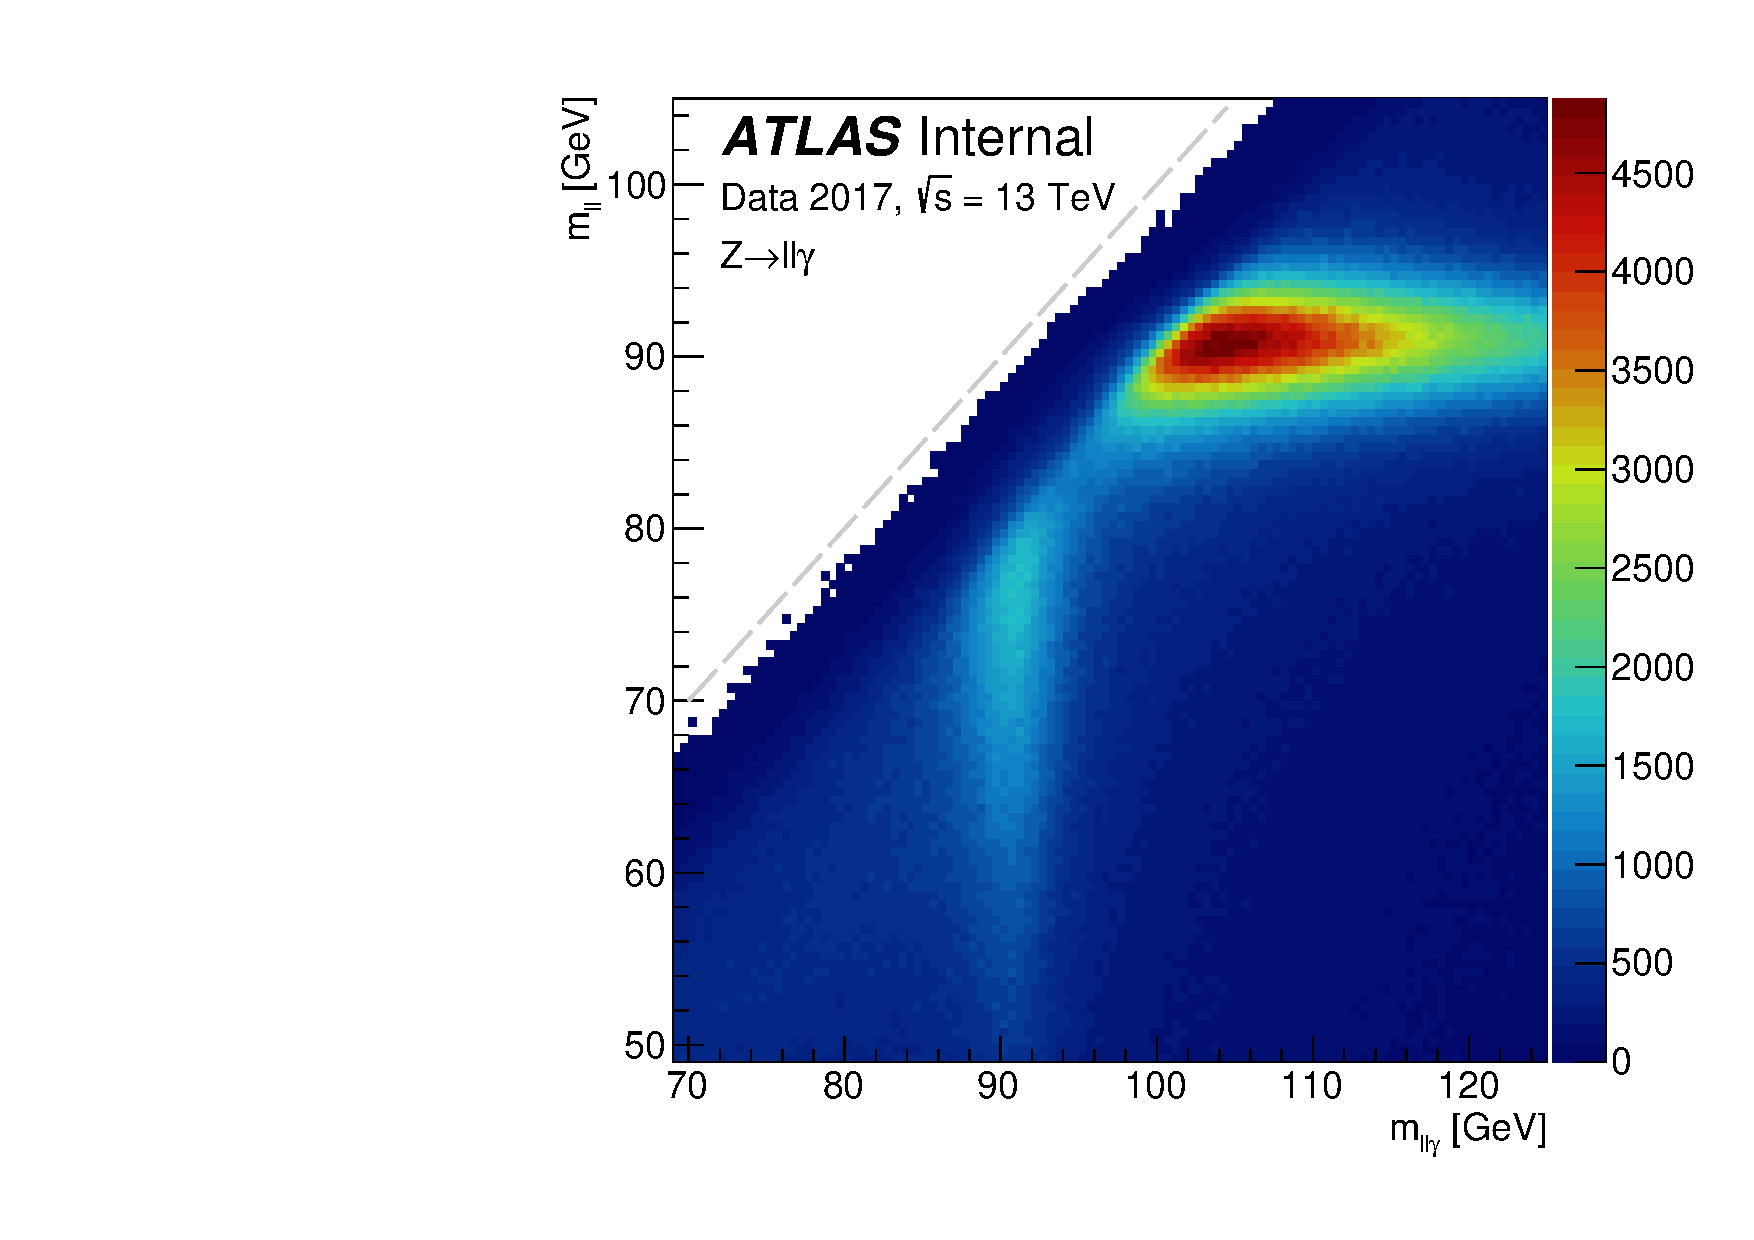
\includegraphics[width=0.5\textwidth]{images/h_mllg_mll.pdf}

  \label{mllgmll}
\end{figure}

La incertidumbre estadística para la eficiencia se obtiene como el intervalo de confianza de un estimador de Bayes con el método de Jeffrey \cite{jeffrey} \commentred{estudiar!}. Las incertezas sistemáticas se obtienen a partir de las variaciones en las eficiencias al modificar algunas de las selecciones. El requisito sobre las masas invariantes se varió de $36<m_{ll}<87$ GeV to $44<m_{ll}<79$ GeV, y de 
$82<m_{ll\gamma}<100$ GeV to $88<m_{ll\gamma}<94$ GeV. Se modificó el requerimiento de identificación de los leptones a \textit{tight} y \textit{medium}, y de aislamiento a \textit{FCTight}.

En la Figura \ref{trigEff} se pueden observar los resultados de las eficiencias en función de las distintas variables. \commentyellow{Creo que se podría agregar la comparación con BS (que da mas eficiente), puedo aprovechar para mencionar BS y citar alguna tesis que describa este método (joaco).} \commentyellow{Faltaría algún plot más?}



\begin{figure}

	\centering

	\caption{Eficiencias de los triggers de fotones para el año 2018 en función del \pt (izquierda), $\eta$ (centro) y $<\mu>$ (derecha). \commentyellow{Voy a agregar lo mismo pero para el resto de los años} \commentNotaIII}

	\begin{subfigure}[b]{0.32\textwidth}
		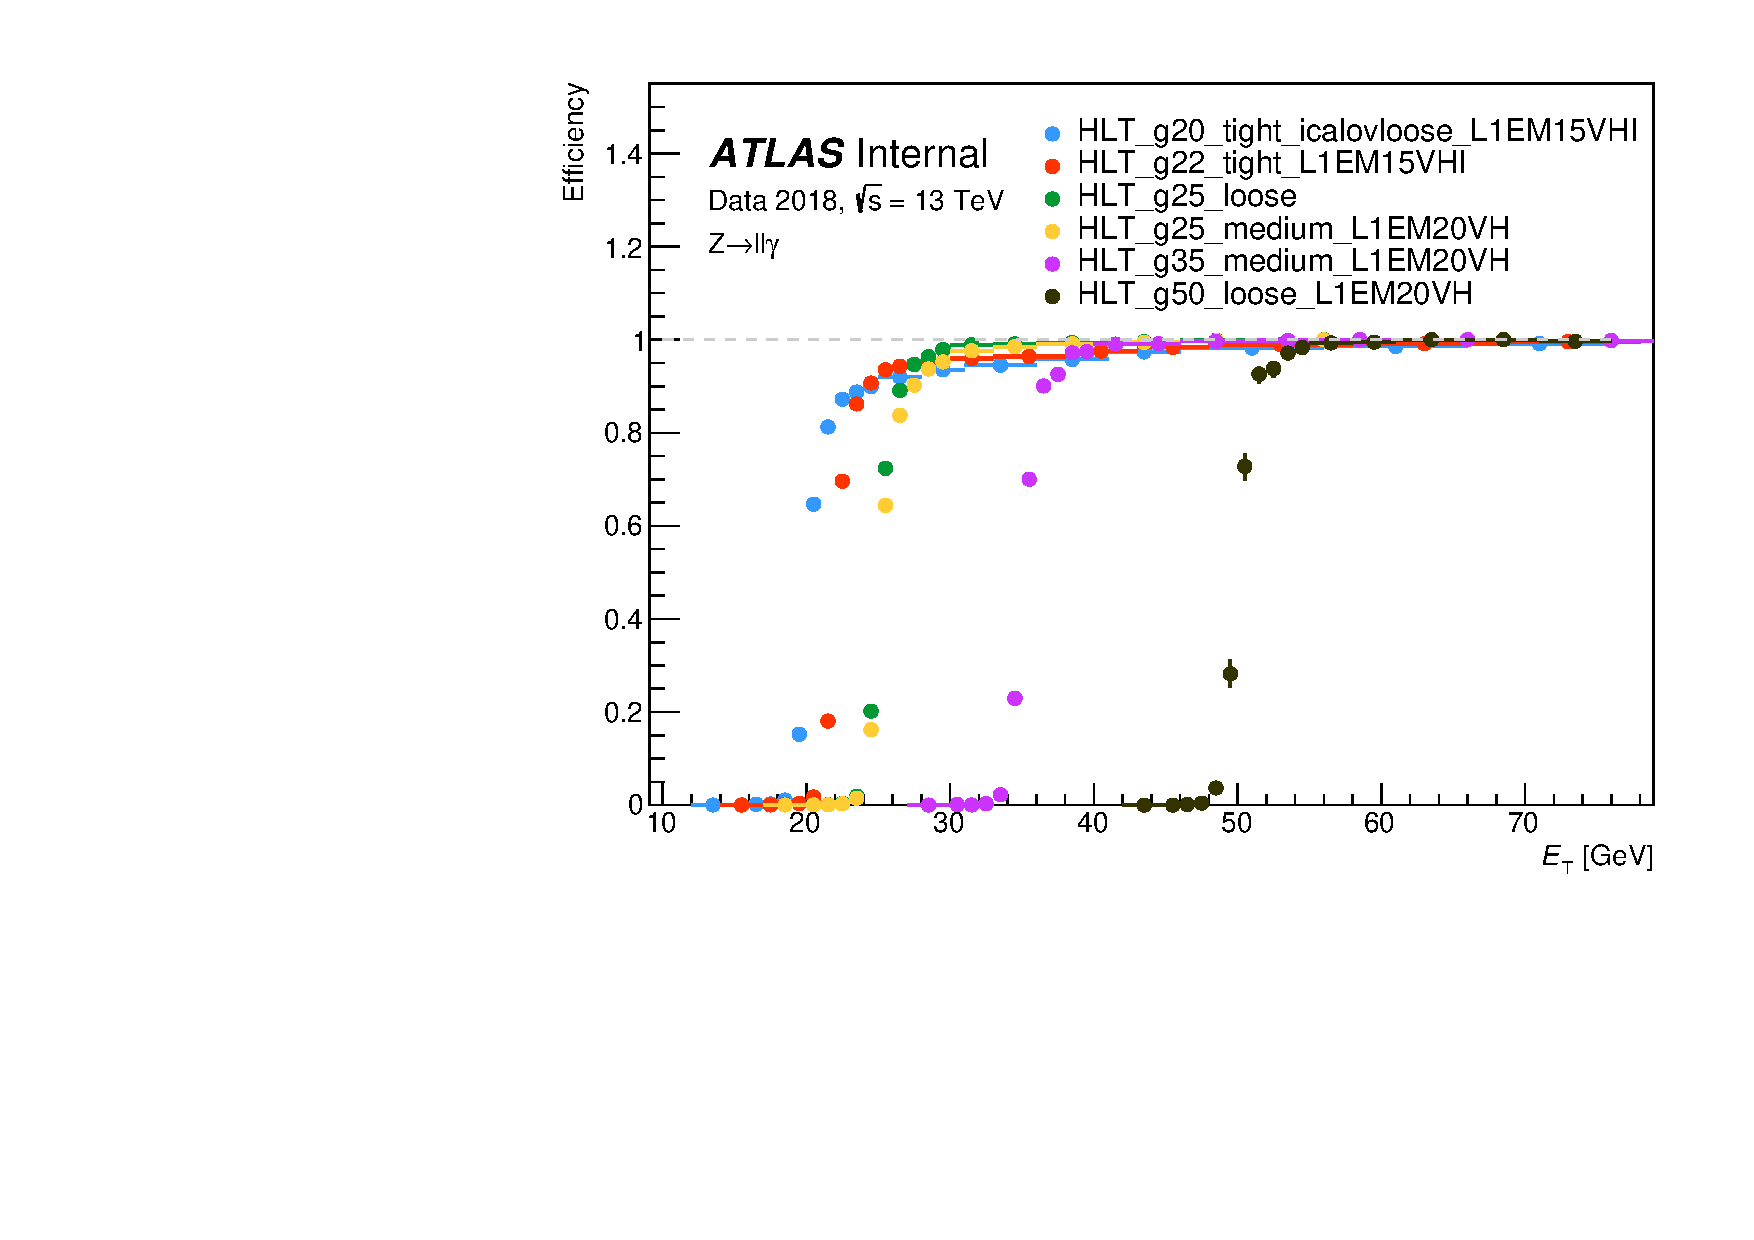
\includegraphics[width=\textwidth]{images/2018_eff_et.pdf}
	\end{subfigure}
	~
	\begin{subfigure}[b]{0.32\textwidth}
		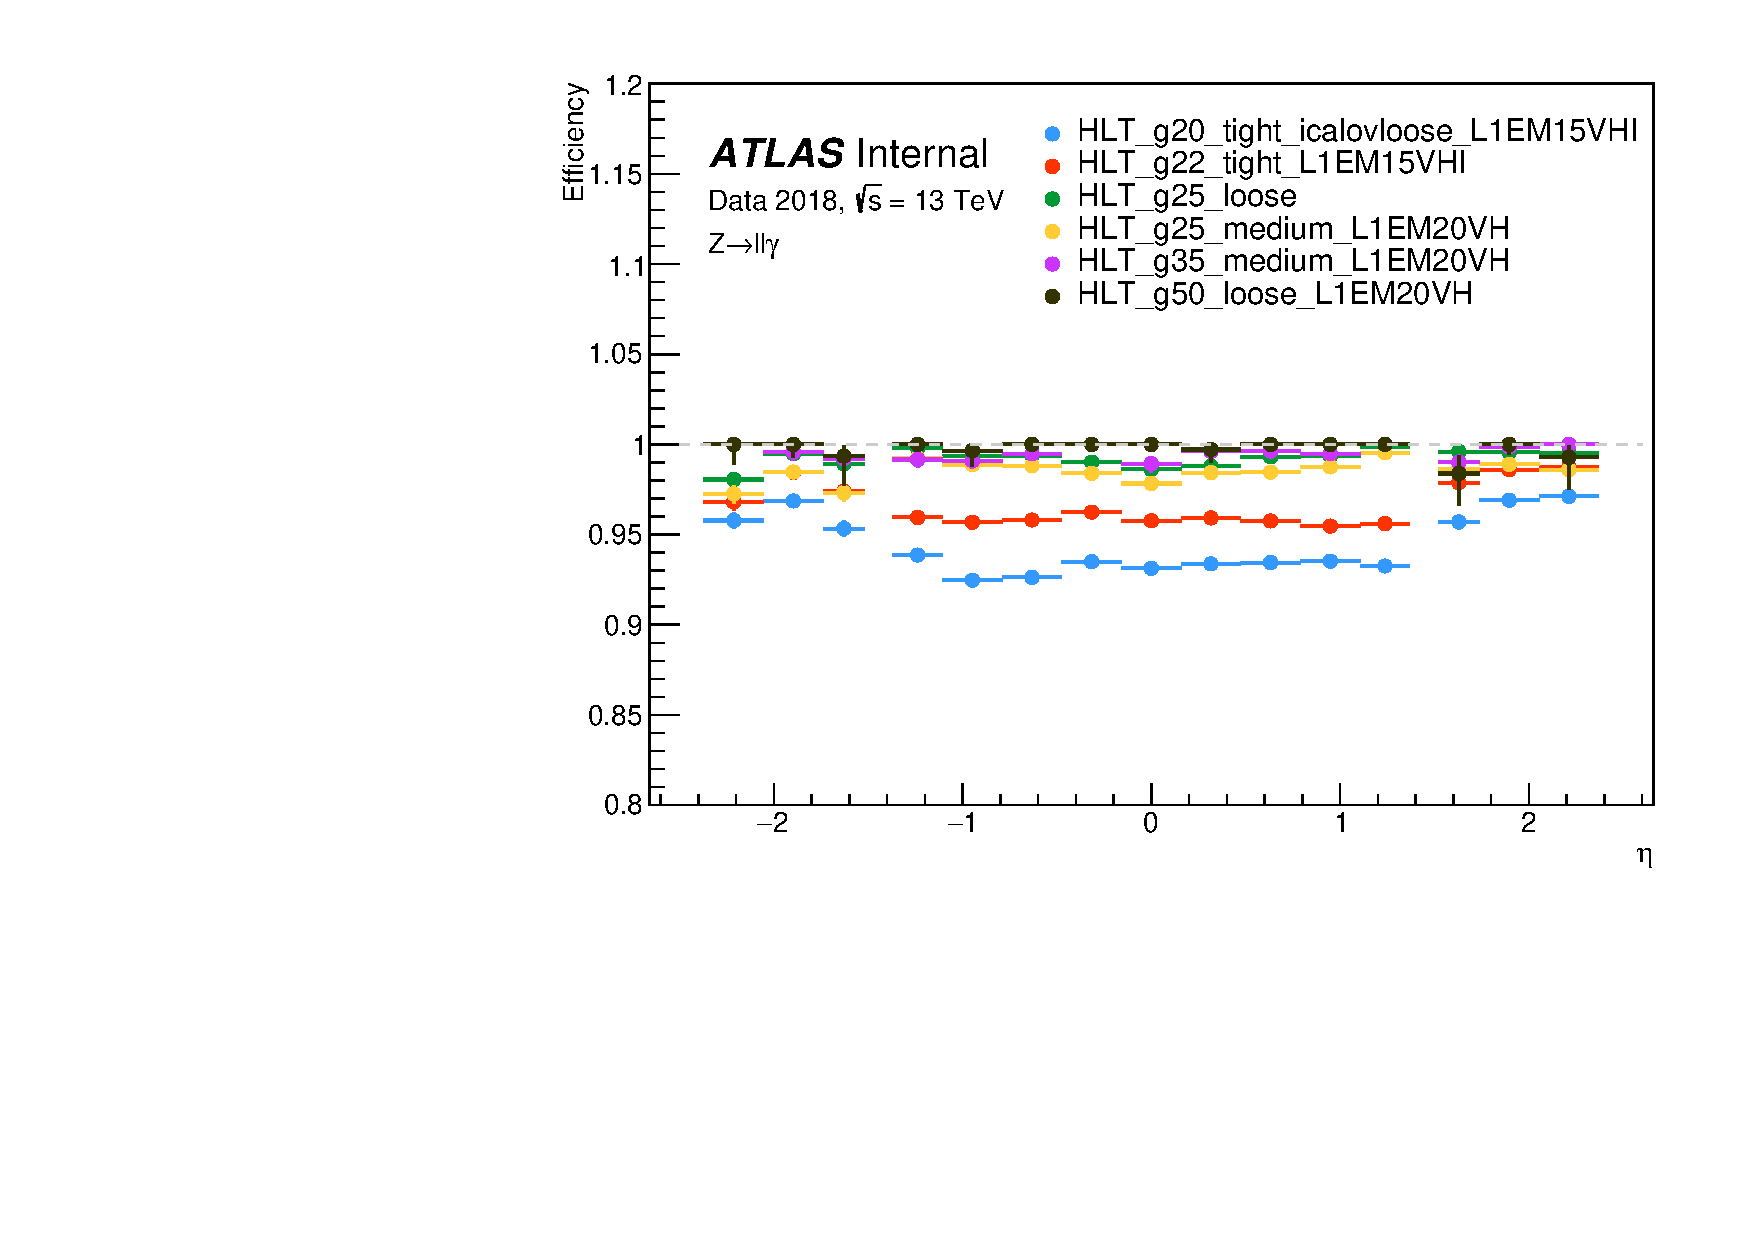
\includegraphics[width=\textwidth]{images/2018_eff_eta_zoom.pdf}
	\end{subfigure}
	~
	\begin{subfigure}[b]{0.32\textwidth}
		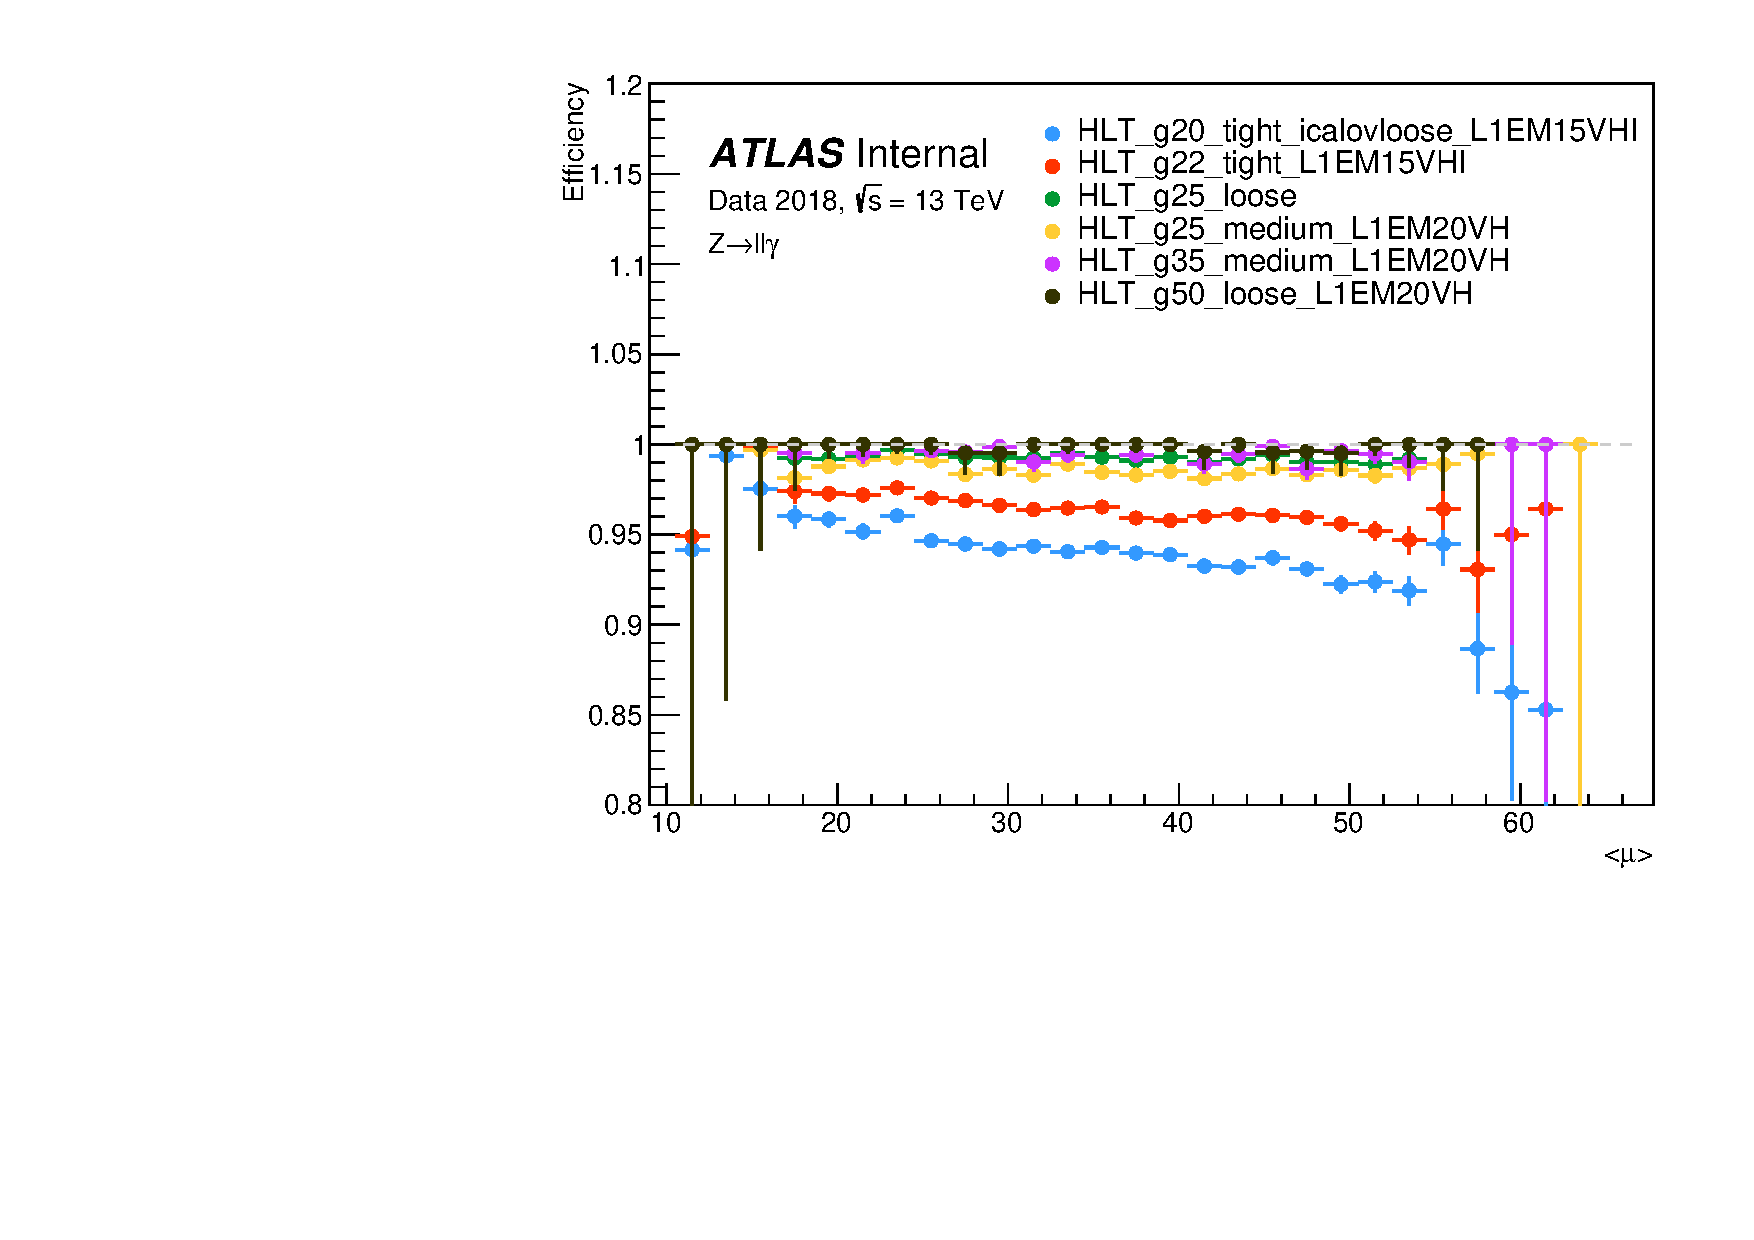
\includegraphics[width=\textwidth]{images/2018_eff_mu_zoom.pdf}
	\end{subfigure}

	\label{trigEff}

\end{figure}


\section{Factores de escala de las eficiencias}

Las simulaciones de Monte Carlo utilizadas en la colaboración son generadas con , aún así no logran reproducir perfectamente los efectos de la interacción entre las partículas y el detector. Estos efectos se traducen en eficiencias en general más altas que las respectivas calculadas con datos, ya que. Con el objetivo de corregir las simulaciones y que se asemejen lo más posible a los datos, se calculan los Factores de Escala (SF). Para el caso de la eficiencia del trigger de fotones, los SFs se definen como el cociente entre las eficiencias calculadas en datos y las calculadas con simulaciones:

\begin{equation}
	\text{SF}(\pt, \eta) = \frac{\epsilon^{\text{(datos)}}(\pt, \eta)}{\epsilon^{\text{(MC)}}(\pt, \eta)}
\end{equation}

En la región con \pt menor al umbral, donde las eficiencias son prácticamente nulas, y en la región del crack se definen los SFs igual $1\pm1$. Las eficiencias de las simulaciones utilizan muestras con procesos con producción de electrones o muones junto con un fotón, y se calculan exactamente de la misma forma que en datos. En la Figura \ref{SFfig} se observa el SF obtenido para el trigger \texttt{HLT\_g25\_loose} con un WP de aislamiento \texttt{FixedCutTightCaloOnly} \commentyellow{Debería agregar todos los plots de SF? No son unos plots muy copados, todo da casi 1 jaja}.


\begin{figure}

	\centering

  \caption{Factor de escala de la eficiencia del trigger \texttt{HLT\_g25\_loose} con un WP de aislamiento \texttt{FixedCutTightCaloOnly} \commentyellow{Había pensado que capaz puedo agregar a la derecha de este plot las eff vs pt y plotear juntos datos y MC, y abajo el ratio que seria el SF.} \commentNotaIII}

  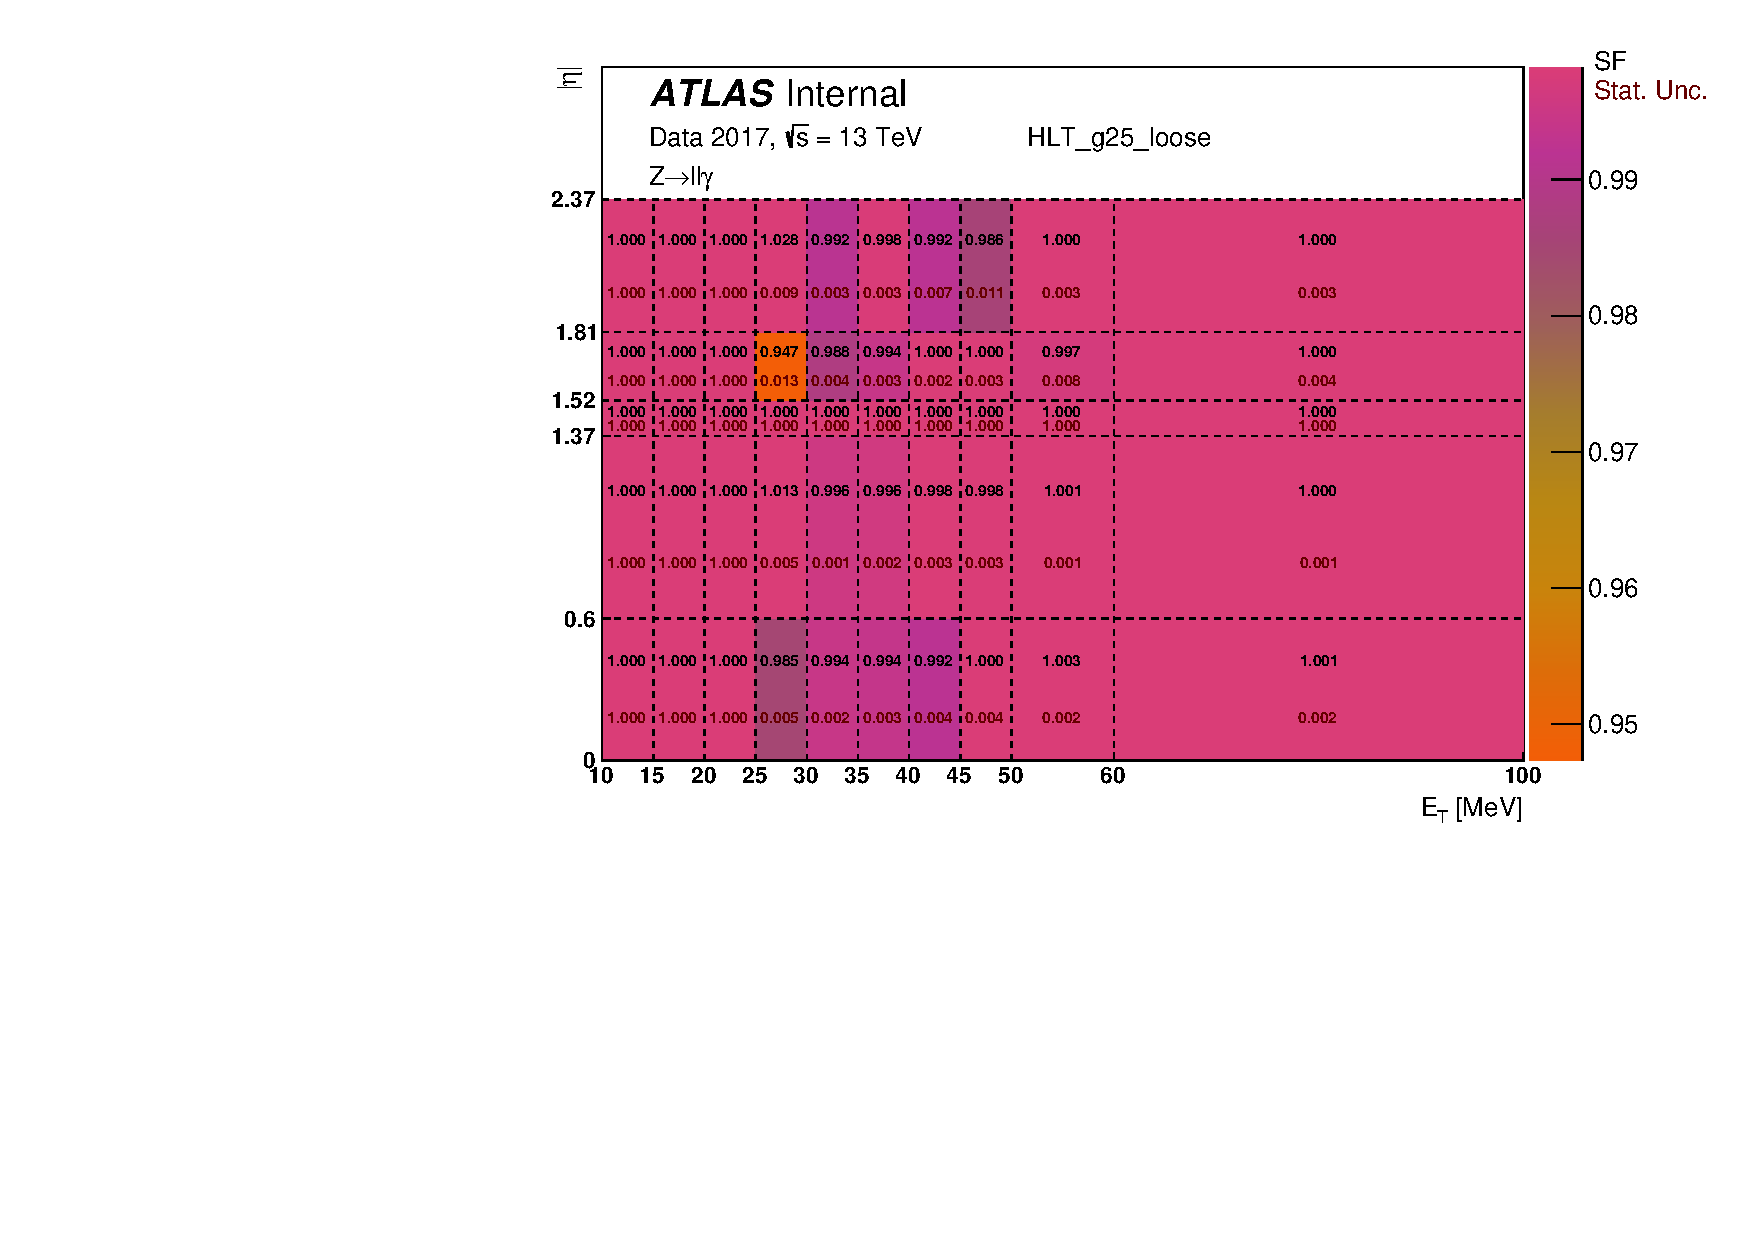
\includegraphics[width=0.5\textwidth]{images/2017_h_sf_et_eta_tr_HLT_g25_loose_FixedCutTightCaloOnly.pdf}

  \label{SFfig}
\end{figure}


